\documentclass{report}
    \title{50004 - Operating Systems - Lecture 6}
    \author{Oliver Killane}
    \date{04/11/21}

%===========================COMMON FORMAT & COMMANDS===========================
% This file contains commands and format to be used by every module, and is 
% included in all files.
%===============================================================================

%====================================IMPORTS====================================
\usepackage[a4paper, total={6in, 8in}]{geometry}
\usepackage{graphicx, amssymb, amsfonts, amsmath, xcolor, listings, tcolorbox, multirow, hyperref}
%===============================================================================

%====================================IMAGES=====================================
\graphicspath{{image/}}

% \centerimage{options}{image}
\newcommand{\centerimage}[2]{\begin{center}
    \includegraphics[#1]{#2}
\end{center}}
%===============================================================================

%=================================CODE LISTINGS=================================
\definecolor{codebackdrop}{gray}{0.9}
\definecolor{commentgreen}{rgb}{0,0.6,0}
\lstset{
    inputpath=code, 
    commentstyle=\color{commentgreen},
    keywordstyle=\color{blue}, 
    backgroundcolor=\color{codebackdrop}, 
    basicstyle=\footnotesize,
    frame=single,
    numbers=left,
    stepnumber=1,
    showstringspaces=false,
    breaklines=true,
    postbreak=\mbox{\textcolor{red}{$\hookrightarrow$}\space}
}

% Create a code listing for a single line
% \codeline{language}{line}{file}
\newcommand{\codeline}[3]{\lstinputlisting[language=#1, firstline = #2, lastline = #2]{#3}}

% Create a code listing for a given language & file
% \codelist{language}{file}
\newcommand{\codelist}[2]{\lstinputlisting[language=#1]{#2}}
%===============================================================================

%================================TEXT STRUCTURES================================
% Marka a word as bold
% \keyword{important word}
\newcommand{\keyword}[1]{\textbf{#1}}

% Creates a section in italics
% \question{question in italics}
\newcommand{\question}[1]{\textit{#1} \\ }

% Creates a box with title for side notes.
% \sidenote{title}{contents}
\newcommand{\sidenote}[2]{\begin{tcolorbox}[title=#1]#2\end{tcolorbox}}

% Creates an item in an itemize or enumerate, with a paragraph after
% \begin{itemize}
%     \bullpara{title}{contents}
% \end{itemize}
\newcommand{\bullpara}[2]{\item \textbf{#1} \ #2}

% Creates a compact list (very small gaps between items)
% \compitem{
%     \item item 1
%     \item item 2
%     \item ...
% }
\newcommand{\compitem}[1]{\begin{itemize}\setlength\itemsep{-0.5em}#1\end{itemize}}

% Creates a link to the lecture for use at the start of the notes document
\newcommand{\lectlink}[1]{\sidenote{Lecture Recording}{
    Lecture recording is available \href{#1}{here}
}}
%===============================================================================


%==============================SYNTAX HIGHLIGHTING==============================
\newcommand{\fun}[1]{\textcolor{blue}{\textbf{#1}}}
\newcommand{\file}[1]{\textcolor{green}{\textbf{#1}}}
\newcommand{\struct}[1]{\textcolor{orange}{\textbf{#1}}}
\newcommand{\var}[1]{\textcolor{purple}{\textbf{#1}}}
\newcommand{\const}[1]{\textcolor{red}{\textbf{#1}}}
%===============================================================================

%==============================THREAD HIGHLIGHTING==============================
\newcommand{\threada}[1]{\textcolor{green}{\textbf{#1}}}
\newcommand{\threadb}[1]{\textcolor{red}{\textbf{#1}}}
%===============================================================================

%============================DISPLAYING THREAD CODE=============================
\newcommand{\threadlist}[3]{
    \codelist{#1}{#2 init.#3}
    \begin{minipage}[t]{0.45\textwidth}
        \codelist{#1}{#2 A.#3}
    \end{minipage}
    \hfill
    \begin{minipage}[t]{0.45\textwidth}
        \codelist{#1}{#2 B.#3}
    \end{minipage}
}
%===============================================================================

\begin{document}
    \maketitle
    \sidenote{Lecture Recording}{
        Lecture recording is available \href{https://imperial.cloud.panopto.eu/Panopto/Pages/Viewer.aspx?id=3bbca698-fdad-477d-8282-add600b793cf}{here}
    }

    \section*{Lock Granularity}
        \begin{minipage}[t]{0.4 \textwidth}
            \codelist{C}{extract coarse.c}
        \end{minipage}
        \begin{minipage}[t]{0.2 \textwidth}
            \begin{huge}
                \[\Rightarrow\]
            \end{huge}
        \end{minipage}
        \begin{minipage}[t]{0.4 \textwidth}
            \codelist{C}{extract fine.c}
        \end{minipage}
        
        \begin{itemize}
            \bullpara{Lock Overhead}{measure of cost associated with a Lock:
                \\ Consider memory use, initialisation cost \& the cost of acquiring and releasing locks.
            }
            \bullpara{Lock Contention}{measure of the number of processes waiting on a lock:
                \\ More contention $\to$ less parallelism
            }
        \end{itemize}
        
        Tradeoffs between fine and coarse grained synchronisation are context dependent, however it is always beneficial to keep critical regions as small as possible.
        \codelist{C}{add account.c}
    \section*{Read/Write Locks}
        For two threads accessing data concurrently we can have race conditions if at least one is changing the shared data.
        \begin{center}
            \begin{tabular}{c r r l}
                && \multicolumn{2}{c}{\textbf{Thread A}} \\
                && read & write \\
                \multirow{2}{*}{\textbf{Thread B}}&read & Safe & Race \\
                &write & Race & Race \\
            \end{tabular}
        \end{center}
        \begin{minipage}[t]{0.4 \textwidth}
            \codelist{C}{viewhistory read.c}
        \end{minipage}
        \begin{minipage}[t]{0.2 \textwidth}
            \
        \end{minipage}
        \begin{minipage}[t]{0.4 \textwidth}
            \codelist{C}{viewhistory write.c}
        \end{minipage}
        \begin{itemize}
            \bullpara{\fun{lock\_RD}}{Acquire the lock in read mode, if another lock has write mode, blocks.}
            \bullpara{\fun{lock\_WR}}{Acquire lock in write mode, if any other thread has the lock in read or write mode, blocks.}
        \end{itemize}
    
    \section*{Memory Models}
        In the course we assume sequential consistency:
        \begin{itemize}
            \item Operations in each thread occur in the order expressed in code/program order.
            \item Operations in each thread are executed in sequential order atomically.
            \item Hence race we can reason more easily about the behaviour of a thread in isolation.
        \end{itemize}
        However there are other memory models (due to compiler optimisations that split up or re-order operations and hardware (e.g core cache coherence)).
        \codelist{C}{weak memory.c}
        \begin{minipage}{0.5 \textwidth}
            \codelist{C}{weak memory A.c}
        \end{minipage}
        \begin{minipage}{0.5 \textwidth}
            \codelist{C}{weak memory B.c}
        \end{minipage}
        Note that we assume a single write is atomic, and immediately visible to threads running on other cpu core, this is typically not the case.
        \\
        \\ Most architectures attempt to be cache coherent (illusion of coherent memory across cores), there are cases where this coherence is not achieved.
        \begin{center}
            \begin{tabular}{c c c c c c}
                \threada{$a = 1$} & \threada{$a = 1$} & \threada{$a = 1$} & \threadb{$b = 2$} & \threadb{$b = 2$} & \threadb{$b = 2$} \\
                \threada{$b = 1$} & \threadb{$b = 2$} & \threadb{$b = 2$} & \threadb{$a = 2$} & \threada{$b = 1$} & \threada{$b = 1$} \\
                \threadb{$b = 2$} & \threada{$b = 1$} & \threadb{$a = 2$} & \threada{$a = 1$} & \threadb{$a = 2$} & \threada{$b = 1$} \\
                \threadb{$a = 2$} & \threadb{$a = 2$} & \threada{$b = 1$} & \threada{$b = 1$} & \threada{$b = 1$} & \threadb{$a = 2$} \\
                $2,2$             & $2,1$             & $2,1$             & $1,1$             & $2,1$             & $2,1$             \\
            \end{tabular}
        \end{center}
        \codelist{C}{flag.c}
        \begin{minipage}{0.5 \textwidth}
            \codelist{C}{flag A.c}
        \end{minipage}
        \begin{minipage}{0.5 \textwidth}
            \codelist{C}{flag B.c}
        \end{minipage}
        With sequential consistency, it is impossible for $flag1 == flag2 == 0$ however under a weak memory model, due to the $if$ statements not being dependent on the assignments, they may be reordered such that this is possible.
    
    \section*{Happens-Before Relationship}
        Formulated by Leslie Lamport in 1976. It is a partial order realtion between events in a trace denoted by $a \to b$ where $a,b$ are events in a trace.
        \sidenote{Partial Order}{
            A partial order is:
            \begin{itemize}
                \bullpara{Irreflexive}{$\forall a .[ a \not\to a]$}
                \bullpara{Antisymmetric}{$\forall a, b . [a \to b \Rightarrow b \not\to a]$}
                \bullpara{Transitive}{$\forall a, b, c .[a \to b \land b \to c \Rightarrow a \to c]$}
            \end{itemize}
        }
        Consider $a$ and $b$ in a trace where $a$ occurs before $b$.
        \begin{itemize}
            \item if $a,b$ are in the same thread, then $a \to b$.
            \item if $a,b$ are not in the same thread and $a : unlock(L)$ and $b : lock(L)$ then $a \to b$ (cannot lock until it is unlocked by other thread.)
        \end{itemize}
        There are other orderings deducible from the synchronisation primitives.
        A \keyword{Race Condition} occurs between $a$ and $b$ iff:
        \compitem{
            \item the access the same memory location
            \item at least one is a write
            \item they are unordered according to \keyword{Happens-Before}
        }
        \codelist{C}{weak memory.c}
        \begin{minipage}{0.5 \textwidth}
            \codelist{C}{weak memory A.c}
        \end{minipage}
        \begin{minipage}{0.5 \textwidth}
            \codelist{C}{weak memory B.c}
        \end{minipage}
        \begin{center}
            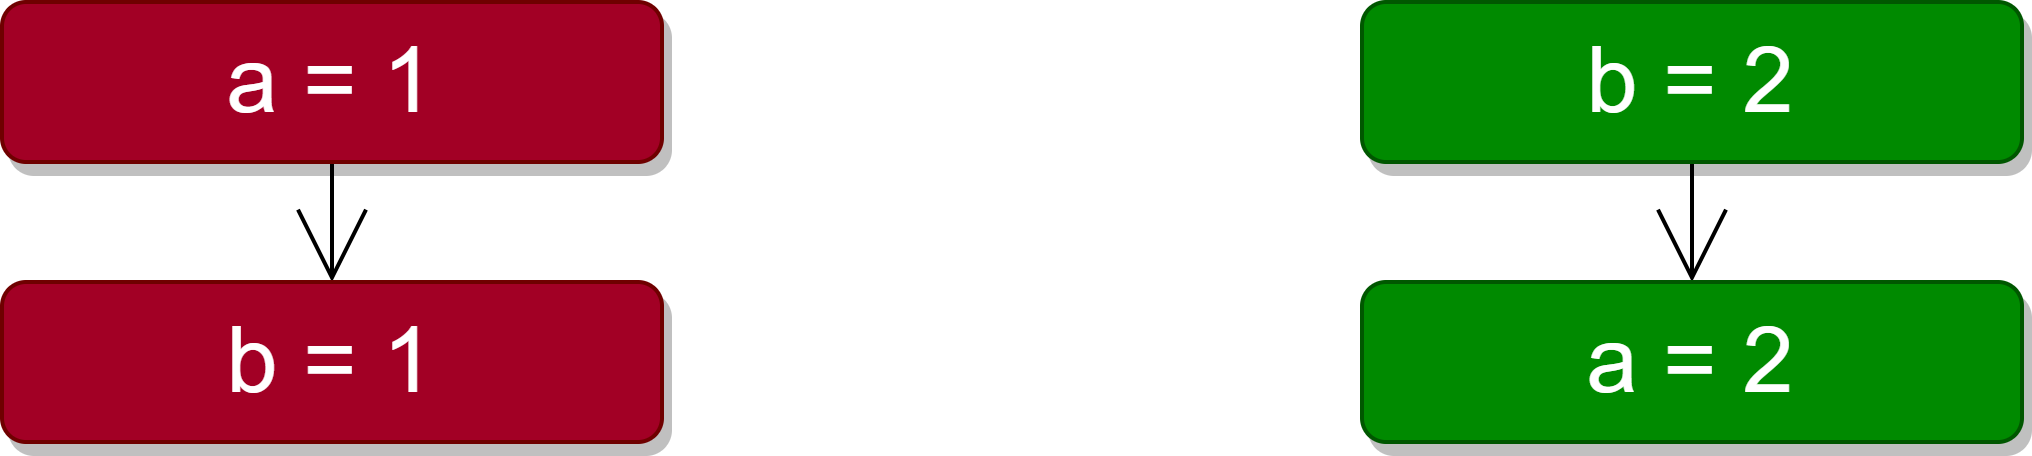
\includegraphics[width=0.5\textwidth]{weak happends-before.png}
        \end{center}
        Hence there is a data race between $a = 1, a = 2$ and $b = 2, b = 1$
        \\ \begin{minipage}{0.5 \textwidth}
            \codelist{C}{weak memory A lock.c}
        \end{minipage}
        \begin{minipage}{0.5 \textwidth}
            \codelist{C}{weak memory B lock.c}
        \end{minipage}
        Two possible execution traces would be:
        \begin{center}
            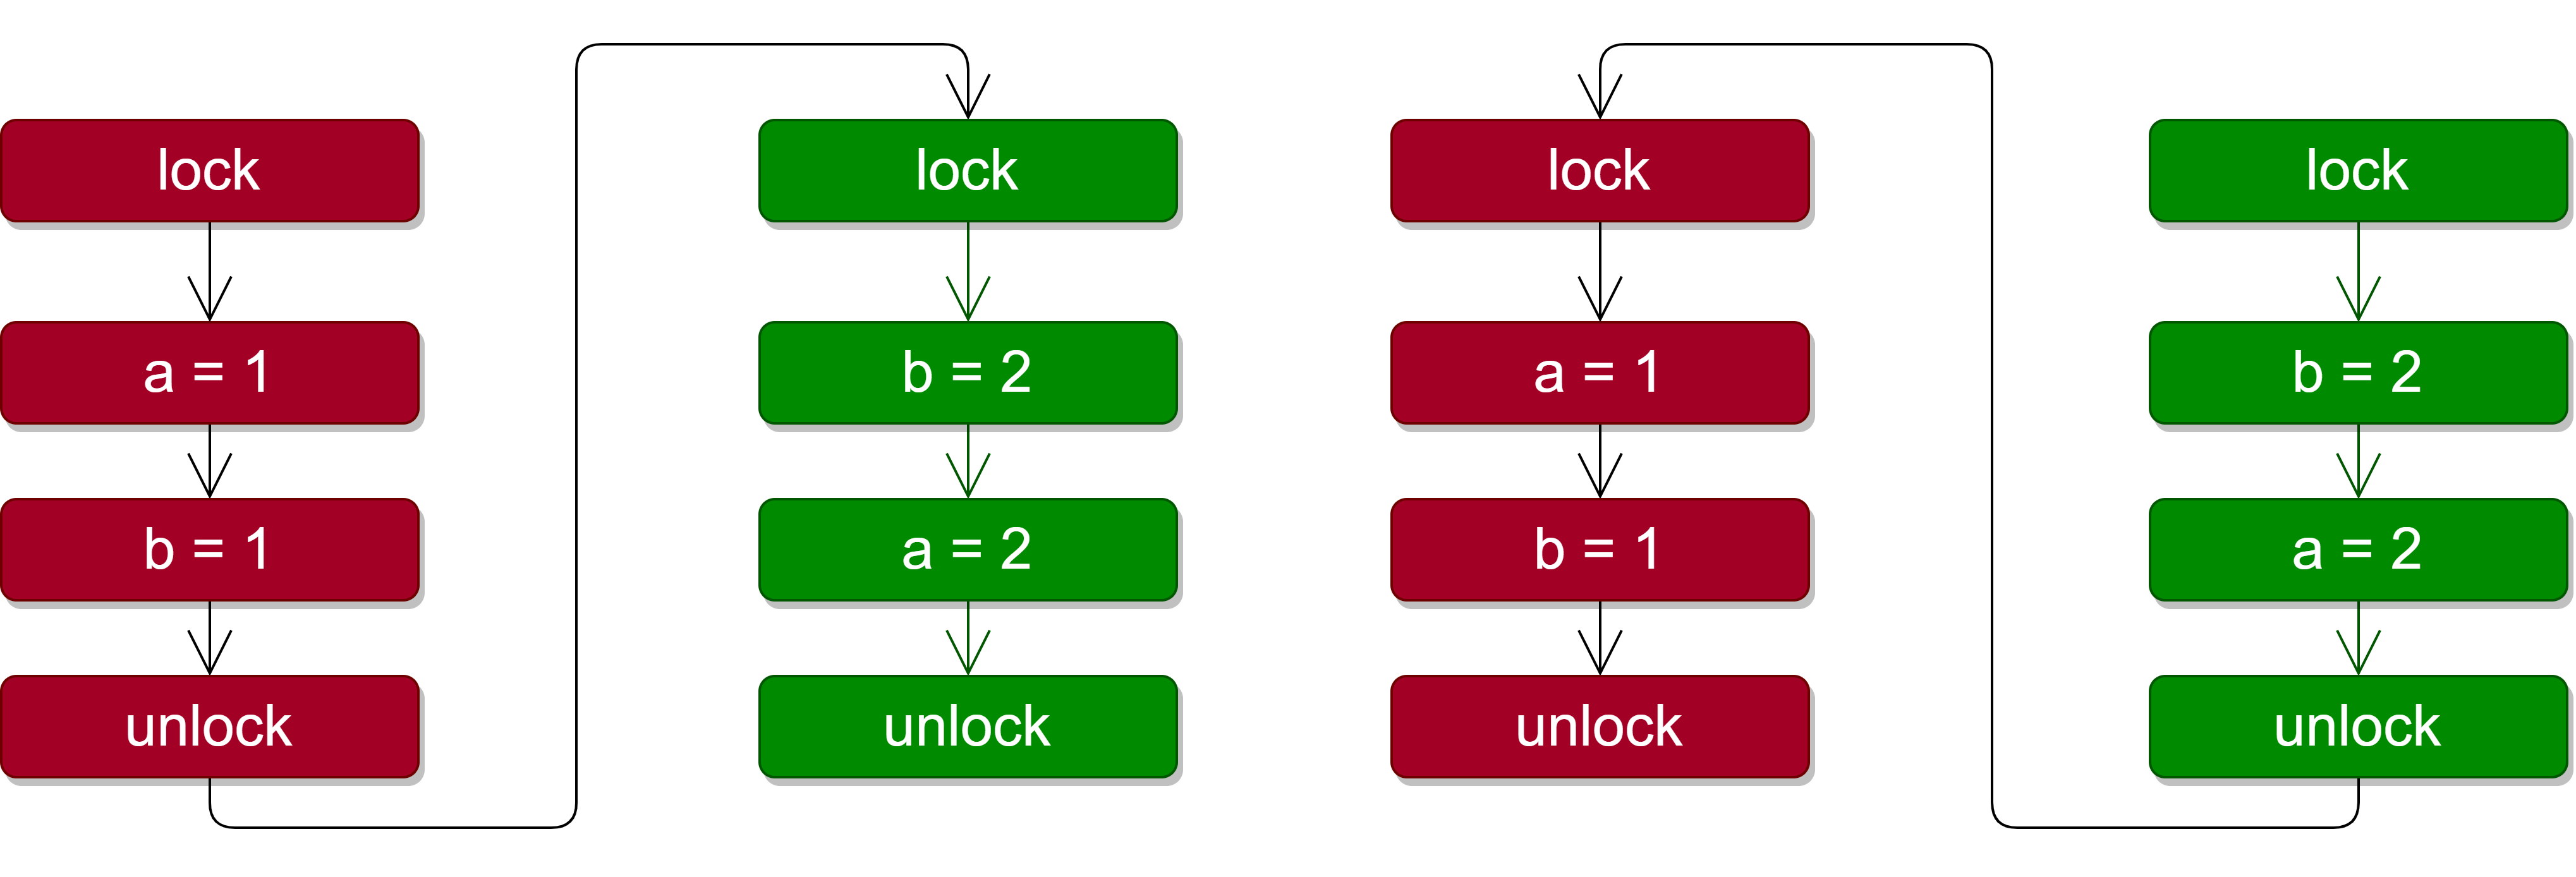
\includegraphics[width=\textwidth]{weak lock happends-before.png}
        \end{center}
        There are no race conditions in either.
        \\ \begin{minipage}{0.5 \textwidth}
            \codelist{C}{weak memory A incr lock.c}
        \end{minipage}
        \begin{minipage}{0.5 \textwidth}
            \codelist{C}{weak memory B incr lock.c}
        \end{minipage}
        \begin{center}
            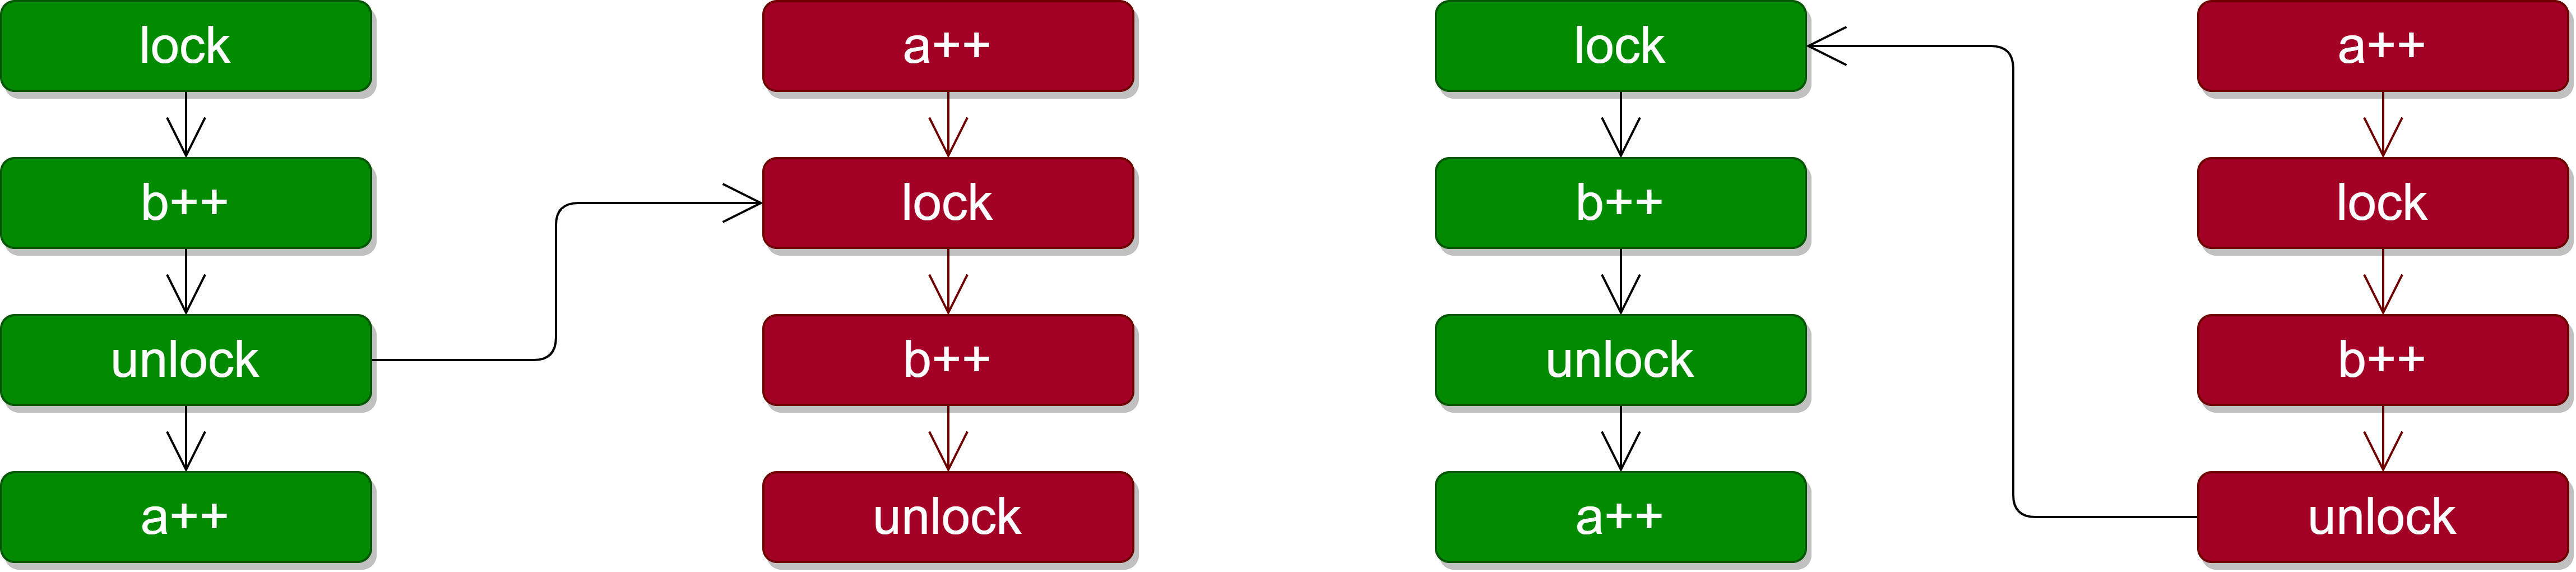
\includegraphics[width=\textwidth]{weak lock incr happends-before.png}
        \end{center}
        Notice that while the right execution trace has no race condition, the left does.
\end{document}
